\newpage{}

\section{Conclusion}
\label{sec:conclusion}
\paragraph{}
\par To finish our work, one can take a look at a direct comparison between the input and output impedences and the resulting gain in decibels obtained through a theoretical analysis and a simulation analysis using Ocatve and Ngspice, respectevely. One can see that the differences are not too significative.

\begin{table}[H]
	\begin{minipage}{.5\linewidth}
		\centering
		\begin{tabular}{|c|c|}
		\hline
		\input{../mat/TOTAL.tex}
		\end{tabular}
		\caption{Theoretical Analysis}
		\label{table1a}
	\end{minipage}
	\begin{minipage}{.5\linewidth}
		\centering
		\begin{tabular}{|c|c|}
		\hline
		\input{../sim/zin_TAB.tex}
		\input{../sim/zout_TAB.tex}
		\input{../sim/results_TAB.tex}
	\end{tabular}
		\caption{Simulation Analysis}
		\label{table1b}
	\end{minipage} 
\end{table}


\begin{figure}[H]
	\includegraphics[width=0.5\linewidth]{gain.eps}
	\centering
	\caption{Gain plot - $\frac{V_o(f)}{V_i(f)}$}
	\label{pha}
\end{figure}

\begin{figure}[H]
    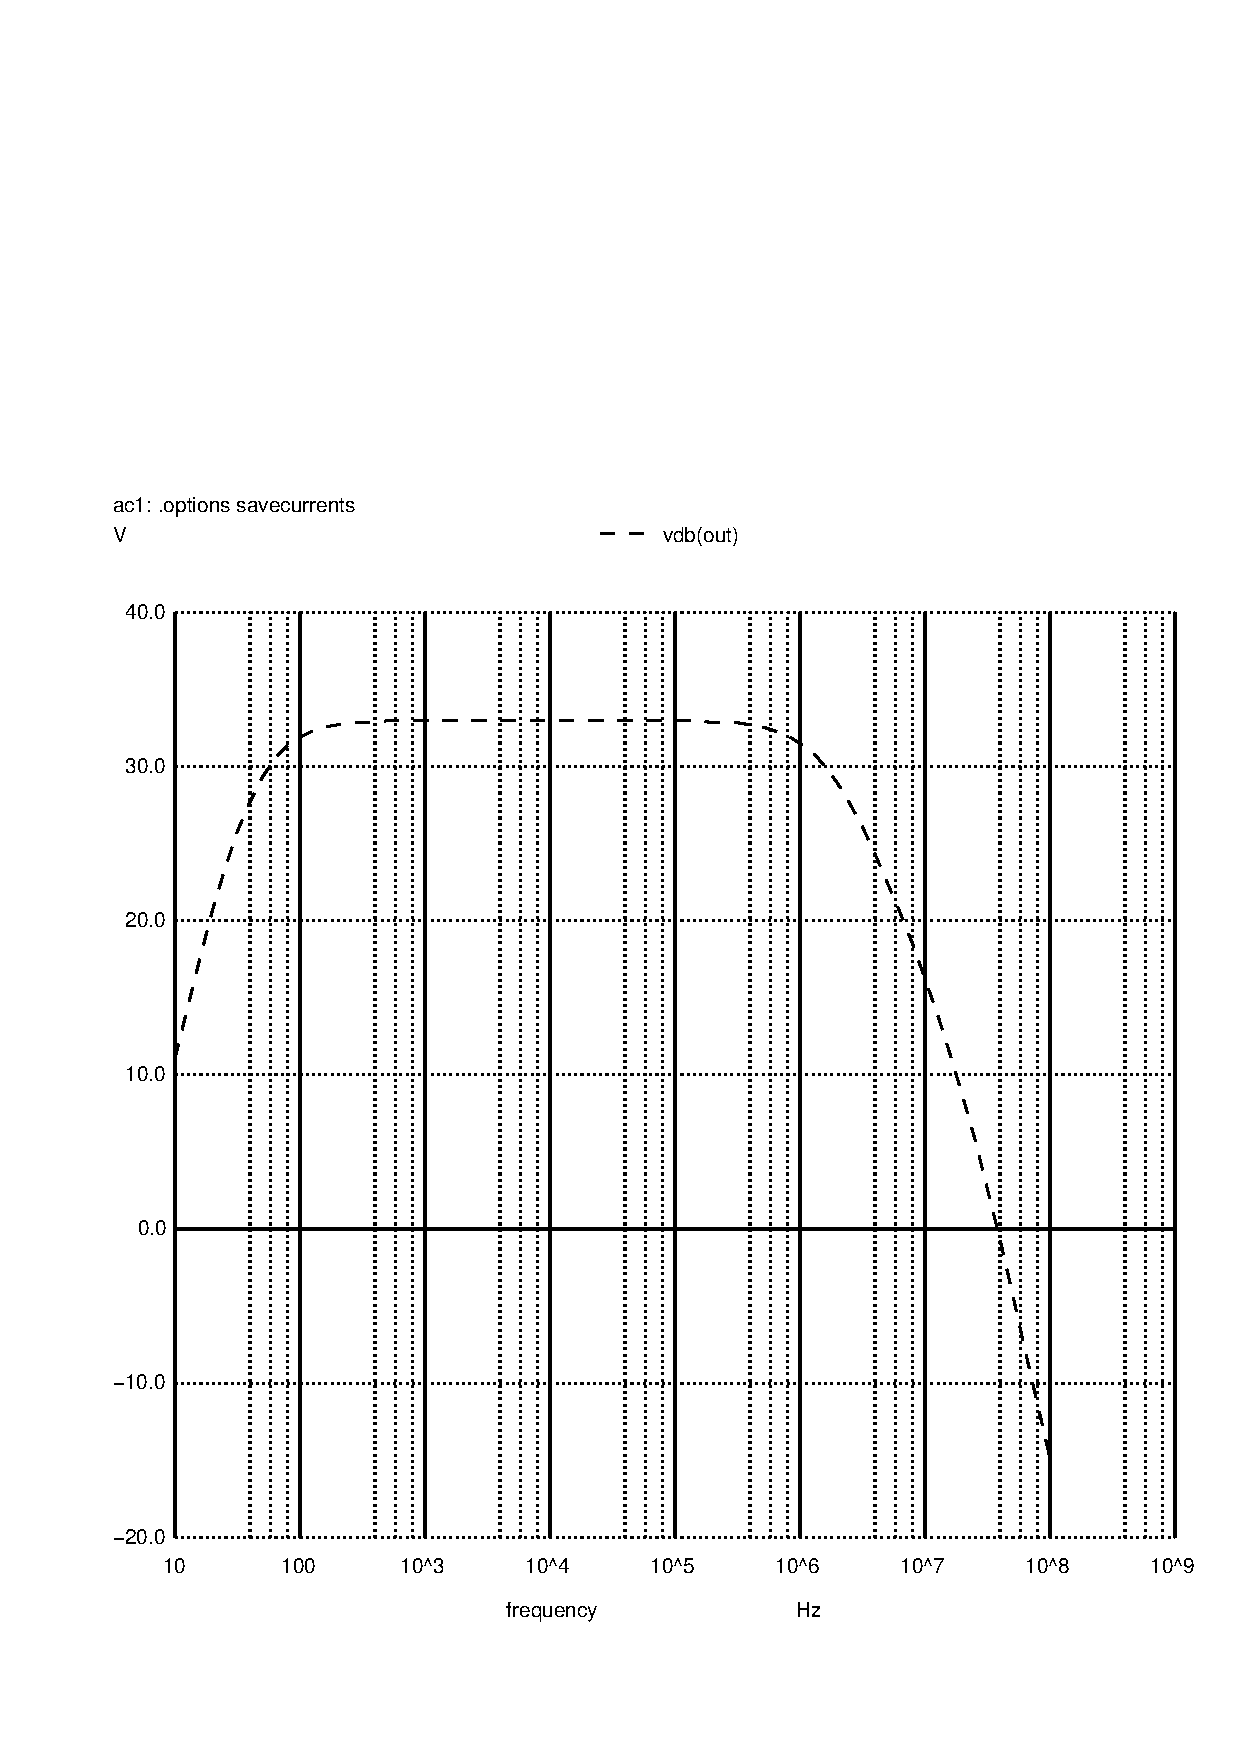
\includegraphics[width=0.495\linewidth]{../sim/vo2f.pdf}
    \centering
    \caption{$v_0-12$ (Deviation from the desired DC voltages)}
    \label{mag}
\end{figure}

\par To sum it all up, we believe the main goal of this lab assignment was achieved: to design an audio amplifier that has the greatest amount of gain possible, spending as little as possible. In both our calculations, the voltage gain is satisfactory when compared to the resources' cost.
\par The greatest boundary came with trying to obtain similar results in both simulations, because the values are significantlly different, like it was observed in the beginning of this conclusion. The main reason for this setback is the non-linear behaviour of the transistors, which interferes with the theoretical calculations, splitting them apart from the simulation values.
\par All in all, both results still satisfy our goals and objectives as the figure of Merit has a valuable considered acceptable by the group.




